\chapter{The Gaussian Process}\label{chap:theory}

\section{Probability Theory}
The reader is assumed to be already comfortable with basic probability theory. Some concepts are nevertheless included here, mainly to introduce the mathematical notation we will use throughout this thesis. 

\subsection{Probability Distributions}
We use $p(X)$ to denote the probability distribution of the random variable $X$, regardless of $X$ being discrete or random. Whether $p(X)$ refers to the \textit{\acrfull{pdf}} for continous random variables or \textit{\acrfull{pmf}} for discrete random variables therefore depend on the context. 

For the probability of a specific event occuring, we will use the notation $\Pr\{X=x\}$ and $\Pr\{X \leq x\}$ instead. This is always a real number, i.e. $\Pr\{\cdot\} \in (0, 1)$. 

\subsection{Joint Distribution}

\subsection{Conditional Distribution}
We use the notation $A | B$ to express the event $A$ occurring given the known occurrence of $B$. In the context of probability distributions, we use $p(A | B)$ for the probability of $A$ occurring, given that we know $B$ has happened.

\subsection{Interpretation of Probability}
We will heavily rely on a Bayesian interpretation of probability in this thesis. Without going into unnecessary philosophical details, the Bayesian view interprets probabilities as beliefs rather than relative frequencies\footnote{The interpretation of probabilities as the relative frequency of outcomes from repeated trials is what is often taught in statistics courses and is called the \textit{frequentist} interpretation.}. 
The benefit of the Bayesian interpretation is that it naturally can be used to model uncertainty of events which we cannot easily express as repeated trials. Examples include one-off events and parameter estimation of fixed but unknown quantities.\footnote{As a thought experiment, let us say you want to determine the number of trees on the planet. There is a fixed amount of trees, but the actual number is unknown as you cannot count every single one. There is nothing uncertain about the number of trees itself, only your beliefs which are uncertain due to incomplete knowledge.} \cite{murphy}.

Central to the Basian view of probability is \textit{Bayes rule}, which is used to update our beliefs $\boldsymbol{\theta}$ when we get new observations $\mathcal{D}$, given by

\begin{equation}
    p(\boldsymbol{\theta} | \mathcal{D}) = \frac{p(\boldsymbol{\theta} \cap \mathcal{D})}{p(\mathcal{D})} = \frac{p(\mathcal{D} | \boldsymbol{\theta}) p(\boldsymbol{\theta})}{p(\mathcal{D})}
\end{equation}
where $p(\boldsymbol{\theta})$ is our prior belief about $\boldsymbol{\theta}$ before observing $\mathcal{D}$, $p(\mathcal{D} | \boldsymbol{\theta})$ is the likelihood of observing $\mathcal{D}$ given a fixed value for $\boldsymbol{\theta}$, $p(\mathcal{D})$ is a normalization constant and $p(\boldsymbol{\theta} | \mathcal{D})$ is our \textit{posterior} beliefs about $\boldsymbol{\theta}$ after observing $\mathcal{D}$. 




\section{The Multivariate Gaussian Distribution}
The Gaussian Distribution is one one the most used distributions in statistics \cite{murphy} and generalizes well for multivariate variables. The pdf for the $D$ dimensional multivariate Gaussian is given by \cref{eq:multivariate_gaussian} \cite{murphy,rasmussen}.
\begin{equation}\label{eq:multivariate_gaussian}
    \mathcal{N}(\boldsymbol{x} \; | \; \boldsymbol{\mu}, \boldsymbol{\Sigma}) \triangleq \frac{1}{(2 \pi)^{D/2} |\boldsymbol{\Sigma} | ^{1/2}} \exp \bigg[- \frac{1}{2} (\boldsymbol{x} - \boldsymbol{\mu})^\intercal \boldsymbol{\Sigma}^{-1}(\boldsymbol{x} - \boldsymbol{\mu})\bigg]
\end{equation}
\subsection{Marginalization and conditioning}
Consider the joint multivariate Gaussian distribution for two (potentially vector-valued) variables $\boldsymbol{x}$ and $\boldsymbol{y}$. 
\begin{equation}
    p(\boldsymbol{x}, \boldsymbol{y}) = \mathcal{N}\bigg(\begin{bmatrix}
        \boldsymbol{x} \\ \boldsymbol{y}
    \end{bmatrix} \; \bigg| \; \begin{bmatrix}
        \boldsymbol{\mu}_x \\ \boldsymbol{\mu}_y
    \end{bmatrix}, \begin{bmatrix}
        \boldsymbol{\Sigma_{xx}} &
        \boldsymbol{\Sigma_{xy}} \\
        \boldsymbol{\Sigma_{yx}} &
        \boldsymbol{\Sigma_{yy}}
    \end{bmatrix}\bigg)
\end{equation}
The marginal and posterior conditional distribution are given by \cref{eq:multivariate_gaussian_marginal} and \cref{eq:multivariate_gaussian_conditional} respectively \cite{rasmussen}, and will be used extensively throughout this thesis.
Note that the marginal distribution do not actually require any calculations and is found by selecting the corresponding values from $\boldsymbol{\mu}$ and $\boldsymbol{\Sigma}$. 
\begin{tcolorbox}[ams align, title={Marginal Distribution}]\label{eq:multivariate_gaussian_marginal}
    p(\boldsymbol{x}) = \int_{\boldsymbol{y}} p(\boldsymbol{x}, \boldsymbol{y}) d\boldsymbol{y} = \mathcal{N}(\boldsymbol{x} \; | \; \boldsymbol{\mu}_x, \boldsymbol{\Sigma}_{xx})
\end{tcolorbox}

 \begin{tcolorbox}[title={Posterior Conditional Distribution}]
 \begin{subequations}\label{eq:multivariate_gaussian_conditional}
 \begin{align}
    p(\boldsymbol{x} | \boldsymbol{y}) &= \mathcal{N}(\boldsymbol{x} \; | \; \boldsymbol{\mu}_{x|y}, \boldsymbol{\Sigma}_{x|y})\\
    \boldsymbol{\mu}_{x|y} &= \boldsymbol{\mu}_x + \boldsymbol{\Sigma}_{xy}\boldsymbol{\Sigma}_{yy}^{-1}(\boldsymbol{y} - \boldsymbol{\mu}_y)\\
    \boldsymbol{\Sigma}_{x|y} &= \boldsymbol{\Sigma}_{xx} -\boldsymbol{\Sigma}_{xy}\boldsymbol{\Sigma}_{yy}^{-1}\boldsymbol{\Sigma}_{yx}
 \end{align}
 \end{subequations}
 \end{tcolorbox}


\section{Introduction to Gaussian Processes}\label{sec:gp}

This introduction is heavily inspired by \cite{rasmussen} where more details can be found for those interested. During this introduction, we will only focus on the scalar case and delay the discussion of vector-valued functions until \cref{sec:theory_vector_gp}. Rest assured, this introduction easily extends to vector-valued functions!

A \acrfull{gp} can formally be defined as Definition \ref{def:gp}.

\newtheorem{gp_def}{Definition}
\begin{gp_def}\label{def:gp}
A Gaussian Process is a collection of random variables, any finite number of which has a joint Gaussian Distribution.
\end{gp_def}

In this thesis we will use a more specific definition in order to interpret \acrshort{gp}'s as a statistical distribution over functions. A \acrshort{gp} for a random function $f \triangleq f(\boldsymbol{x})$ is fully specified by its mean function $m(\boldsymbol{x})$ and covariance function $k(\boldsymbol{x}, \boldsymbol{x}')$.

\begin{equation}\label{eq:gp}
    f \sim GP(\;m(\boldsymbol{x}), \; k(\boldsymbol{x}, \boldsymbol{x}')\;)
\end{equation}

This interpretation of a \acrshort{gp} might seem a bit odd at first. The key observation is that the marginal distribution $p(\boldsymbol{x})$ of a multivariate Gaussian distribution $p(\boldsymbol{x}, \boldsymbol{y})$ is another Gaussian distribution that is completely independent of $\boldsymbol{y}$, as expressed in \cref{eq:multivariate_gaussian_marginal}. Any variables not of interest can therefore easily be marginalized away, leaving only the subset of variables we care about.

Any \acrshort{gp} by Definition \ref{def:gp} can therefore be viewed as the finite marginal distribution of an infinite Gaussian Distribution, jointly describing the values of $f$ at all possible inputs $\boldsymbol{x}$. In the end, a \acrshort{gp} is nothing more than a joint Gaussian Distribution with a fancy interpretation.

\subsection{A quick note on vector notation}
Different notations for vector values is used to differentiate between three common cases:
\begin{description}
\item[Bold letters] are used to indicate a single, multivariate value. $f(\boldsymbol{x})$ is the scalar function $f$ evaluated at the multivariate input $\boldsymbol{x}$. In practice, this implies the input is $\boldsymbol{x} \in \mathcal{R}^{1 x M}$ with $M\geq 2$ columns. 
\item[Capital letters] such as $X$, are used to indicate multiple (potentially multivariate) samples. $f(X)$ is the scalar function $f$ evaluated at each row in $X$. In practice this implies that the input $X \in \mathcal{R}^{N x M}$ with $N \geq 2$ rows (samples) and $M \geq 1$ columns (dimensions).
\item[Vector Arrow] such as $\vec{f}$ is used to denote vector-fields (i.e. vector-valued functions). This will be useful when we get to vector-valued \acrshort{gp}s, and allow the distinction between shorthand notations such as $\boldsymbol{f}_* = f(X_*)$, $\vec{f}_* = \vec{f}(\boldsymbol{x}_*)$ and $\vec{\boldsymbol{f}}_* = \vec{f}(X_*)$.
\end{description}

\subsection{Introduction to kernels}
The covariance function $k(\boldsymbol{x}, \boldsymbol{x}')$ determines the similarity between two different points $\boldsymbol{x}$ and $\boldsymbol{x}'$. These covariance functions will in this thesis be referred to as a \textit{kernel}, which maps the input space to a \textit{feature-space} \cite{rasmussen}. The output of the kernel is a value describing the similarity (i.e., covariance) between the two inputs. Kernel functions are discussed in greater detail in \cref{sec:kernels}.

The kernel must be positive definite to produce a valid covariance matrix, which requires that

\begin{equation}
    k(\boldsymbol{x}, \boldsymbol{x}') = k(\boldsymbol{x}', \boldsymbol{x})
\end{equation}

The covariance matrix $K(X, X)$ is the result of calling $k(\cdot, \cdot)$ on all pairs on inputs, i.e.
\begin{equation} 
    K(X, X)_{ij} = k(\boldsymbol{x}_i, \boldsymbol{x}_j) \quad \forall i, j
\end{equation}

\subsection{Conditioning}
So far, we have only specified the prior distribution for $f$. As a \acrshort{gp} is by definition a multivariate Gaussian Distribution, the posterior conditional in \cref{eq:multivariate_gaussian_conditional} can be used to condition $f$ on observed values. 
As an example, we use a simple \acrshort{gp} for $f$ with mean $m$ and kernel $k$.

Let $\boldsymbol{f}_* \triangleq f(X_*)$ denote the function evaluated at test points $X_*$. Before any observations are made we can only rely on prior information as shown in \cref{fig:gp_prior}. From a Bayesian perspective, we want to update our prior beliefs about $\boldsymbol{f}_*$ after observing noisy values $\boldsymbol{y} = f(X) + \epsilon$ at multiple inputs $X$ to get the posterior belief $p(\boldsymbol{f}_* \; | X, \boldsymbol{y}, X_*)$.

The joint distribution of $\boldsymbol{y}$ and $\boldsymbol{f}_*$ is given by 

\begin{equation}
    p(\boldsymbol{y}, \boldsymbol{f}_*) = \mathcal{N}\bigg(\begin{bmatrix}
        \boldsymbol{y} \\ \boldsymbol{f}_*
    \end{bmatrix} \; \bigg| \begin{bmatrix}
        m(X) \\ m(X_*)
    \end{bmatrix},  \begin{bmatrix}
        K(X, X) + \sigma I & K(X, X_*) \\ K(X_*, X) & K(X_*, X_*)
    \end{bmatrix}\bigg)
\end{equation}

The posterior distribution $p(\boldsymbol{f}_* | \boldsymbol{y})$ can easily be computed using the posterior conditional distribution in \cref{eq:multivariate_gaussian_conditional}.
\begin{subequations}\label{eq:gp_conditional}
\begin{align}
    p(\boldsymbol{f}_* | \boldsymbol{y}) &= \mathcal{N}(f \; | \; \boldsymbol{\mu}_{\boldsymbol{f}_*|\boldsymbol{y}}, \boldsymbol{\Sigma}_{\boldsymbol{f}_*|\boldsymbol{y}})\\
    \mathbb{E}[\boldsymbol{f}_*] =  \boldsymbol{\mu}_{\boldsymbol{f}_* | \boldsymbol{y}} &= m(X_*) + K(X_*, X) \; \big(K(X, X) + \sigma I\big)^{-1} \; (\boldsymbol{y} - m(X))\label{eq:gp_conditional_mean}\\
    \mathbb{V}[\boldsymbol{f}_*] = \boldsymbol{\Sigma}_{\boldsymbol{f}_* | \boldsymbol{y}} &= K(X_*, X_*) - K(X_*, X)  \big(K(X, X) + \sigma I\big)^{-1} \; K(X, X_*)\label{eq:gp_conditional_var}
\end{align}
\end{subequations}

As the notation quickly gets messy for the general case, we also introduce a shorthand notation for evaluating $f(\boldsymbol{x}_*)$ at a single test point, which is what we most often want. To follow the convention used by \cite{rasmussen}, we introduce $\boldsymbol{k}_* \triangleq K(X, \boldsymbol{x}_*)$ as a vector of covariances calculated between the test point and each of the training samples, as well as $K \triangleq K(X, X)$ and $\bar{f}_* \triangleq \mathbb{E}[f_*]$. Using this shorthand notation for a single test case, \cref{eq:gp_conditional} boils down to \cref{eq:gp_conditional_simple}.

\begin{subequations}\label{eq:gp_conditional_simple}
\begin{align}
    \bar{f}_* = \mathbb{E}[f_*]  &= m(\boldsymbol{x}_*) + \boldsymbol{k}_*^\intercal ( K + \sigma I)^{-1} (\boldsymbol{y} - m(X))\\
    \mathbb{V}[f_*] &= k(\boldsymbol{x}_*, \boldsymbol{x}_*) - \boldsymbol{k}_*^\intercal K^{-1} \; \boldsymbol{k}_*\label{eq:gp_conditional_var_simple}
\end{align}
\end{subequations}

In practice, computing the inverse $K(X, X)$ becomes expensive for an increasing number of samples. To avoid numerical instability, using the \textit{Cholesky Decomposition} is usually preferred. The Cholesky Decomposition forms a new lower-triangular matrix $L$ such that $K = L L^\intercal$, and can be seen as the matrix equivalent of the square root. \cref{eq:gp_conditional} can then be computed using $L$. The diagonal entry $\sigma I$ added to the kernel matrix is intended to model noisy observations. However, it also improves the numerical stability, so a small value is recommended even if the observations are noise-free \cite{scikit-learn}.
\begin{subequations}
\begin{align}
    \begin{split}
    \mathbb{E}[{\boldsymbol{f}}_*] &= m(X_*) + K(X_*, X) \; (L L^\intercal)^{-1} \; (\boldsymbol{y} - m(X))\\ &= m(X_*) + K(X_*, X) \; \underbrace{\big[(L^\intercal)^{-1} (L)^{-1}  \; (\boldsymbol{y} - m(X))\big]}_{\boldsymbol{\alpha}}
    \end{split}\\
    \begin{split}
    \mathbb{V}[\boldsymbol{f}_*] &= K(X_*, X_*) - K(X_*, X) \; (L L^\intercal)^{-1} \; K(X, X_*)\\
    &= K(X_*, X_*) - K(X_*, X) \; (L^\intercal)^{-1} (L)^{-1} \; K(X, X_*)\\
    &= K(X_*, X_*) - \underbrace{\big[(L)^{-1} \; K(X, X_*)\big]^\intercal}_{\boldsymbol{v^\intercal}} \; \underbrace{\big[(L)^{-1} \; K(X, X_*)\big]}_{\boldsymbol{v}}
    \end{split}
\end{align}
\end{subequations}

This boils down to \cref{alg:gp_prediction} as proposed by \cite{rasmussen}. A simple \acrshort{gp} before and after conditioning is shown in \cref{fig:gp_simple}

\begin{algorithm}[H]
\begin{algorithmic}[1]
\Procedure{GP-PREDICT}{$X_*$, $\boldsymbol{y}$, $k$, $X$}
    \State $L = cholesky\big(K(X, X) + \sigma I\big)$
    \State $\boldsymbol{\alpha} = L^\intercal \backslash (L \backslash \boldsymbol{y})$
    \State $\boldsymbol{v} = L \backslash K(X, X_*)$
    \State $\bar{\boldsymbol{f}}_* = m(X_*) + K(X_*, X) \boldsymbol{\alpha}$
    \State $\mathbb{V}[\boldsymbol{f}_*] = K(X_*, X_*) - \boldsymbol{v}^\intercal \boldsymbol{v}$
\EndProcedure
\end{algorithmic}
\caption{Gaussian Process Prediction}
\label{alg:gp_prediction}
\end{algorithm}

\begin{figure}[h]
    \centering
    \begin{subfigure}{0.49\textwidth}
        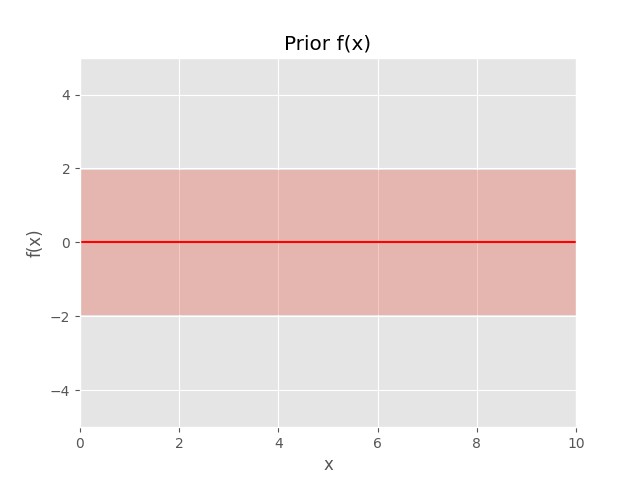
\includegraphics[width=\textwidth]{figures/introduction-gp/prior.png}
        \caption{Prior}
        \label{fig:gp_prior}
    \end{subfigure}
    \begin{subfigure}{0.49\textwidth}
        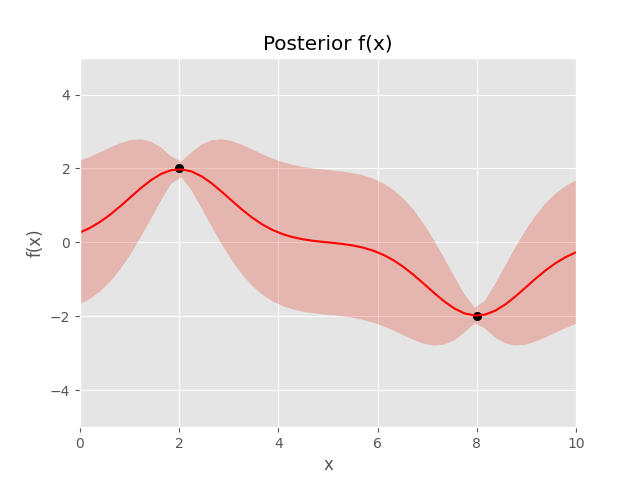
\includegraphics[width=\textwidth]{figures/introduction-gp/posterior.png}
        \caption{Posterior after observing the function at two different inputs (black dots).}
        \label{fig:gp_posterior}
    \end{subfigure}
    \caption{Simple Gaussian Process example with zero-mean and \acrshort{rbf} kernel with unit variance. The red line is the mean, while the red area is the $95\%$ confidence interval.}
    \label{fig:gp_simple}
\end{figure}

\section{Vector-valued Gaussian Process}\label{sec:theory_vector_gp}
\acrshort{gp}s can easily be extended for vector-valued functions by simply considering the joint distribution of each function component as in \cref{eq:gp_vector}. In this thesis we will assume independent components, i.e. $k_{xy}=k_{yx}=0$
\begin{equation}\label{eq:gp_vector}
     \vec{f}(\boldsymbol{x}) = \begin{bmatrix} f_x (\boldsymbol{x})\\ f_y (\boldsymbol{x})\end{bmatrix} \sim \text{GP} \big(\begin{bmatrix} m_x(\boldsymbol{x})\\m_y(\boldsymbol{x})\end{bmatrix}, \ \begin{bmatrix}
    k_{xx}(\boldsymbol{x}, \boldsymbol{x}') & k_{xy}(\boldsymbol{x}, \boldsymbol{x}') \\ k_{xy}(\boldsymbol{x}, \boldsymbol{x}')^\intercal & k_{yy}(\boldsymbol{x}, \boldsymbol{x}')
    \end{bmatrix}\big) 
\end{equation}

\section{Kernels}\label{sec:kernels}
This section will introduce some relevant kernels for this thesis. However, many more kernels are available in the literature. 
\subsection{Stationary Kernels}
Stationary kernels are kernels which only depends on $\boldsymbol{r} = \boldsymbol{x} - \boldsymbol{x'}$ and is usually specified as a function of a single variable.
\subsubsection{Constant Kernel}
As the name implies, the constant kernel is a kernel that is independent of the input.

\begin{equation}
    k(\boldsymbol{\cdot}) = \sigma^2
\end{equation}

\subsubsection{White kernel}
The \textit{White Kernel} is useful for modeling whitenoise in a system as independently and identically normally distributed \cite{scikit-learn}. Note that adding this kernel is similar, but not identical to the noise term added to the training kernel in \cref{alg:gp_prediction}, as this kernel also affect the prediction input. 
\begin{equation}
    k(\boldsymbol{r}) = \delta (r) \sigma^2
\end{equation}

\subsubsection{Radial Basis Function}\label{sec:kernels_rbf}
The \textit{\acrfull{rbf}} kernel, also referred to as \textit{squared exponential kernel}, is one of the most frequently used kernels, and is given by the covariance function in \cref{sec:kernels_rbf}. The scaling parameter $l$ is the \textit{charactheristic length scale} and can intuitively be thought of as a smoothness parameter. This kernel yields infinitely differentiable functions, meaning that any functions drawn from a \acrshort{gp} with this kernel are very smooth\cite{rasmussen}.
\begin{equation}\label{eq:kernel_rbf}
    k(\boldsymbol{r}) = \exp \big\{-\frac{||\boldsymbol{r}||^2}{2 l^2}\big\}
\end{equation} 

\subsubsection{Matérn class}
The \textit{Matérn Class} of kernels are given by the covariance function in \cref{eq:kernel_matern}, where $K_v$ is the \textit{modified Bessel function}. 

\begin{equation}\label{eq:kernel_matern}
    k(\boldsymbol{r}) = \frac{2^{1-v}}{\Gamma(v)}\bigg(\frac{\sqrt{2 v} ||\boldsymbol{r}||}{l} \bigg)^v K_v \bigg(\frac{\sqrt{2v} || \boldsymbol{r}||}{l} \bigg)
\end{equation}
The parameter $v > 0$ determines the smoothness, where:
\begin{itemize}
    \item $v=\frac{1}{2}$ yields the \textit{Ornstein-Uhlenbeck Process} and functions, that when drawn from a \acrshort{gp} with this kernel, are continious, but not differentiable. The kernel is equivalent to $$k(\boldsymbol{r}) = \exp \{-\frac{||\boldsymbol{r}||}{l}\}$$
    \item $v=\frac{3}{2}$ yields functions that, when drawn from a \acrshort{gp} with this kernel, are continous and once-differentiable. The kernel is equivalent to $$k(\boldsymbol{r}) = \big(1 + \frac{\sqrt{3} ||\boldsymbol{r}||}{l}\big) \exp\big\{- \frac{\sqrt{3} ||\boldsymbol{r}||}{l}\big\}$$
    \item $v=\frac{5}{2}$ yields functions, that when drawn from a \acrshort{gp} with this kernel,  are continous and twice differentiable. The kernel is equivalent to $$k(\boldsymbol{r}) = \big(1 + \frac{\sqrt{5} ||\boldsymbol{r}||}{l} + \frac{5 ||\boldsymbol{r}||^2}{3 l^2}\big) \exp\big\{- \frac{\sqrt{5} ||\boldsymbol{r}||}{l}\big\}$$
\end{itemize}
More generally, the functions drawn from a \acrshort{gp} with a Matérn class kernel, is $k$-times differentiable if and only if $v > k$\cite{rasmussen}. The Matérn class of kernels is argued to be a better choice than the \acrshort{rbf} kernel for many physical systems, as the infinitely smooth function generated by \acrshort{rbf} is too smooth \cite{rasmussen}.
Further mathematical details can be found in \cite[sec.~4.2]{rasmussen} as it is outside the scope of this thesis.


\subsection{Combining multiple kernels}
Kernels can be mixed and matched through multiplication and addition, where the behavior of the individual kernels can be combined to describe more complex functions. A simple example is using the constant kernel to scale the covariance of other functions. Kernels can also be applied to only specific input dimensions in order t
\section{Hyperparameter selection}
Manually tuning the kernel hyperparameters is tedious and time-consuming, motivating the need for automatic selection of parameters. In this section, we will introduce a few practical methods for model selection with \acrshort{gp}s.

\subsection{Maximum Likelihood - The Marginal Likelihood}\label{sec:gp_mle}
The \textit{marginal likelihood}, the likelihood of observing a set of given observations $\boldsymbol{y}$, conditioned on a \acrshort{gp} with kernel parameters $\boldsymbol{\theta}$ and inputs $X$ is given by 

\begin{equation}
    p(\boldsymbol{y} \; | \; X, \boldsymbol{\theta}) = \mathcal{N}\big(\boldsymbol{y} \; | \; \boldsymbol{m}(X), K_{\boldsymbol{\theta}}(X, X)\big)
\end{equation}
and can be used to obtain a \textit{\acrfull{ml}} estimate of the parameters $\boldsymbol{\theta}$.
Defining $\tilde{\boldsymbol{y}} \triangleq \boldsymbol{y} - \boldsymbol{m}(X)$ and taking the logarithm, we get \cref{eq:gp_log_marginal_likelihood} 
\begin{tcolorbox}[ams align, title={Log Marginal Likelihood}]\label{eq:gp_log_marginal_likelihood}
    \begin{split}
    \log p(\boldsymbol{y} \; | \; X, \boldsymbol{\theta}) = &-\frac{1}{2} \tilde{\boldsymbol{y}}^\intercal K_{\boldsymbol{\theta}}(X, X)^{-1}\tilde{\boldsymbol{y}} - \frac{1}{2} \log |K_{\boldsymbol{\theta}}(X, X)| \ldots\\ &- \frac{n}{2} \log (2 \pi)
    \end{split}
\end{tcolorbox} where the optimal hyperparameters $\boldsymbol{\theta}_{\text{ML}}$ can be found by maximizing this quantity\footnote{
    The marginal likelihood is generally not a convex function of $\boldsymbol{\theta}$ as the kernel functions usually are non-linear functions of $\boldsymbol{\theta}$, and multiple local optima may exist. The practical effects include that the observed data may be explained well by different combinations of parameters, and each combination serves as a distinct interpretation of the data. During optimization, care should be taken to avoid a bad local optimum \cite{rasmussen}.}, i.e.
\begin{equation}
    \boldsymbol{\theta}_{\text{ML}} = \arg \max_{\boldsymbol{\theta}} \log p(\boldsymbol{y} \; | \; X, \boldsymbol{\theta}) = \arg \min_{\boldsymbol{\theta}} \big(- \log p(\boldsymbol{y} \; | \; X, \boldsymbol{\theta})\big)
\end{equation}

The name \textit{marginal likelihood} comes from the fact that the latent function $\boldsymbol{f}$ is marginalized out, i.e. we are really optimizing the parameters over all possible latent functions $\boldsymbol{f}$.

\begin{equation}
    p(\boldsymbol{y} \; | \; X, \boldsymbol{\theta}) = \int_{\boldsymbol{f}} p\big(\boldsymbol{y} \;| \; \boldsymbol{f}\big) p\big(\boldsymbol{f} \; |\; m(X), K(X, X)\big) d\boldsymbol{f}
\end{equation}

\section{Sampling from a Gaussian Process}\label{sec:gp_samples}
As the \acrshort{gp} is a jointly Gaussian distribution, we can draw random samples from it as with any other multivariate Gaussian.

\begin{equation}\label{eq:gp_samples}
    \boldsymbol{f}_* \sim \mathcal{N}(\bar{\boldsymbol{f}}_*, \mathbb{V}[\boldsymbol{f}_*])
\end{equation}

More specifically, we can convert a vector $Z$ of independent and identically distributed standard normal samples into samples from a jointly Gaussian distribution.

Once again, we make use of the Cholesky decomposition to decompose the \acrshort{gp} covariance, i.e. $\mathbb{V}[\boldsymbol{f}_*] = L L^\intercal$. Using $L$ and $\bar{\boldsymbol{f}}_*$, \cref{eq:gp_samples} can be expressed as 
\begin{equation}
    \mathcal{N}(\bar{\boldsymbol{f}}_*, \mathbb{V}[\boldsymbol{f}_*]) = \bar{\boldsymbol{f}}_* + L \mathcal{N}(0, I)
\end{equation}
showing us how we can convert indendent standard normal samples into samples from our \acrshort{gp} \cite{rasmussen}:

\begin{equation}
    \boldsymbol{f}_* = \bar{\boldsymbol{f}}_* + L Z, \quad Z \sim \mathcal{N}(0, I)
\end{equation}

\section{Approximate methods}
The standard derivation of the \acrshort{gp} requires inverting the kernel matrix, either through the Cholesky Decomposition or directly. The computational complexity of the Cholesky decomposition is $\frac{n^3}{6}$ and $\frac{n^2}{2}$ for solving triangular systems \cite{rasmussen}. This may be acceptable for sparse datasets but makes \acrshort{gp}s infeasible for Big Data applications. 

For simple functions, it often works well only to use a representable subset of the data. However, throwing away the majority of available data is not an elegant solution to the problem. 
\subsection{Variational Gaussian Process}

\subsubsection{A short introduction to Variational Inference}\todo[]{This may be a bit out of scope, consider removing}
Variational Inference was covered thoroughly in a previous specialization project \cite{mellbye}. A quick introduction of the necessary concepts is included here, and more details can be found in \cite{mellbye, murphy}.

In many cases, using the true posterior distribution $p(\boldsymbol{\theta} | \mathcal{D})$ turns out to be challenging. Calculating the posterior using Bayes Rule requires a normalizing constant $p(\mathcal{D})$, which quickly becomes infeasible unless the distributions are simple. The true posterior are therefore often assumed only to be known up to a normalizing constant, i.e.

\begin{equation}
    \tilde{p}(\boldsymbol{\theta} | \mathcal{D}) \triangleq p(\mathcal{D} | \boldsymbol{\theta})p(\boldsymbol{\theta}) \propto p(\boldsymbol{\theta} | \mathcal{D})
\end{equation}

An exact analytical solution to the posterior is then unavailable, and one would have to turn to approximate inference methods. 
One such method, \textit{\acrfull{vi}}, approximates the posterior distribution $p(\boldsymbol{\theta} | \mathcal{D})$ with a simpler, \textit{surrogate distribution} $q(\boldsymbol{\theta})$. If we can find a $q(\boldsymbol{\theta})$ similar to $p(\boldsymbol{\theta} | \mathcal{D})$, we can use the simpler surrogate density to perform inference.

To find a good surrogate density $q(\cdot)$ we use the \textit{\acrfull{kl}} as a measure of similarity between the two probability distributions, where the reverse\footnote{\acrshort{kl} is generally not symmetric in its input arguments, i.e. $\mathbb{KL}(p || q) \neq \mathbb{KL}(q || p)$} \acrshort{kl} is given by
\begin{align}
    \mathbb{KL}(q || p) = \int_{\boldsymbol{\theta}} q(\boldsymbol{\theta}) \log \frac{q(\boldsymbol{\theta})}{p(\boldsymbol{\theta})} d\boldsymbol{\theta} = E_{q} \big[ \log \frac{q(\boldsymbol{\theta})}{p(\boldsymbol{\theta})} \big]\label{eq:kl_qp}
\end{align}
As we only know the unnormalized posterior distribution $\tilde{p}$, we cannot actually compute the reverse \acrshort{kl}. However, we can still find the best surrogate density $\hat{q}$ by observing that the argument minimizing $\mathbb{KL}(q || p)$ also minimizes $\mathbb{KL}(q || \tilde{p})$, i.e.

\begin{align}
    \hat{q}(\boldsymbol{\theta}) &= \arg \min_q \mathbb{KL}(q || p)\\ &= \arg \min_q \big(\mathbb{KL}(q || \tilde{p}) + \log p(\mathcal{D})\big) \\&= \arg \min_q \mathbb{KL} (q || \tilde{p})
\end{align}

The best surrogate density can therefore be found by maximizing the \textit{\acrfull{elbo}} given by 
\begin{equation}
    \text{ELBO} \triangleq -\mathbb{KL}(q || \tilde{p})
\end{equation} which can be computed using the unnormalized posterior $\tilde{p}$. If we assume a known parametric representation of $q(\cdot)$, we can then turn the problem of selecting a good surrogate density into an optimization problem of finding the set of parameters maximizing \acrshort{elbo}. 

\subsubsection{Sparse Variational Gaussian Process}
To deal with the computational complexity of \acrshort{gp}s, \cite{Titsias2008VariationalMS} introduced the \textit{\acrfull{svgp}}. A short introduction is included here. 

Rather than directly using all the available training data directly, we can rather attempt to summarize the data $(X, \boldsymbol{y})$ using a set of $m$ \textit{inducing variables} for the latent function values $\boldsymbol{f}_m$ at the inducing points $X_m$. $X_m$ can either be a subset of the available training inputs $X$ or auxiliary \textit{pseudo-points}. The goal of \acrshort{svgp} is then to infer the inducing points $X_m$ as well as the hyperparameters $\boldsymbol{\theta}$ from data.



\subsubsection{}
